
\chapter{Reproducibility of LibKGE framework}
\label{chap:reproducibility}

In their analysis of hybrid training, \citet{chen2021relation} showed that by including negative relation examples to 1vsAll training objective, models could perform better in entity prediction task. Therefore, this chapter will describe our  attempt to reproduce \citet{chen2021relation}'s results using LibKGE framework. 


Table \ref{tab:AKBC results} shows the performance of their best models on entity prediction on FB15K-237 and WN18RR. In the table, \textit{"Entity"} indicates that the type of negative examples are negative entity examples generated by perturbing the subject and object position. While \textit{"Relation"} indicated that negative examples are negative relation examples. \textit{"Yes"} value determines the existence of those corresponding type of negative examples in 1vsAll, while \textit{"No"} value means there is an absence of those types in 1vsAll.

Table \ref{tab:AKBC results} clearly highlights the perquisite of incorporating negative relation examples with negative entity examples into 1vsAll training objective (hybrid training objective). By including negative relation examples,  ComplEx model can achieve the 2\% higher in entity MRR on FB15K-237 dataset. We also observed the improvement of model's performance in entity Hits@\{1, 3, 10\}. However, on WN18RR, the improvement were not significant, ComplEx model can achieve the 0.1\% higher in all of metrics.

\begin{table}[!htbp]
\centering
\resizebox{0.9\textwidth}{!}{
\begin{tabular}{@{}lllllll@{}}
\toprule
\textbf{Dataset}   & \textbf{Entity} & \textbf{Relation} & \textbf{MRR}   & \textbf{Hits@1} & \textbf{Hits@3} & \textbf{Hits@10} \\ \midrule
FB15K-237 & Yes                        & No                           & 36.6          & 27.1           & 40.1           & 55.7            \\
                   & Yes                        & Yes                          & \textbf{38.8} & \textbf{29.8}  & \textbf{42.5}  & \textbf{56.8}   \\
                   & No                         & Yes                          & 26.3          & 18.7           & 28.7           & 41.1            \\  \midrule
WN18RR    & Yes                        & No                           & 48.7          & 44.1           & 50.1           & 58.0            \\
                   & Yes                        & Yes                          & \textbf{48.8} & \textbf{44.3}  & \textbf{50.5}  & \textbf{57.8}   \\
                   & No                         & Yes                          & 25.8          & 21.2           & 29.0           & 33.9            \\ \bottomrule
\end{tabular}
}
\caption[The performance of ComplEx models on test data.]{The performance of ComplEx models in Entity Ranking on Test data. The results are taken from \citep{chen2021relation}'s paper.}
\label{tab:AKBC results}
\end{table}



Although their finding is remarkable, the models' performance on relation prediction was neglected, and the impact of hybrid training on overall MRR (i.e., micro-average of entity MRR and relation MRR) was not examined. Furthermore, how model perform on both entity ranking and relation prediction if we use overall MRR in model selection alongside with hybrid training objective is also an interesting question we attempt to study. 

Therefore, to have fairness in the comparative study (Chapter \ref{chap:comparative_study}), it is essential to reproduce the models found by \citet{chen2021relation} using LibKGE \citep{libkge}. Using LibKGE python-library \citep{libkge} for implementation, we can utilize its modular design, giving us flexibility when designing/running experiments \citep{Ruffinelli2020You}. Furthermore, LibKGE also provides the framework for KGE models; therefore, we can save time and effort on re-implementation.

% We can easily see that factor is a main impact.

\section{Preliminary results on reproducing}

\noindent\textbf{Experimental setup.} In their study, \citet{chen2021relation} conducted experiments with the ComplEx model, the nuclear 3-norm (N3) regularizer and Adagrad optimizer. The model was trained for 400 epochs with a binary cross-entropy (BCE) loss function and 1vsAll. Hyperparameter optimization was conducted using a grid search with five different hyperparameters: embedding size (\textit{d}), learning rate (\textit{lr}), batch size (\textit{bsz}), and the weight of regularizer (\textit{reg}), and weight of relation prediction ($\lambda$). The first four hyper-parameters are shown Table \ref{tab:AKBC grid search}. For WN18RR, the weight of relation prediction ($\lambda$) was searched over \{0.005, 0.001, 0.05, 0.1, 0.5, 1\}. For FB15k-237, \citet{chen2021relation} searched over \{0.125, 0.25, 0.5, 1, 2, 4\}. The best configuration for each of the datasets was chosen based on entity MRR. Table \ref{tab:AKBC best models} shows the best configuration found by \citet{chen2021relation}.

\begin{table}[!htbp]
\centering
\resizebox{\textwidth}{!}{%
\begin{tabular}{@{}lllll@{}}
\toprule
\textbf{Dataset} & \textit{d} \tablefootnote{The embedding size was written follow LibKGE.}            & \textit{lr}     & \textit{bsz}         & \textit{reg}  \\ \midrule
FB15k-237        & \{200, 1000, 2000\} & \{0.1, 0.01\} & \{100, 500, 1000\} & \{0.0005, 0.005, 0.01, 0.05, 0.1, 0.5, 1, 0\} \\ 
WN18RR           & \{200, 1000, 2000\} & \{0.1, 0.01\} & \{100, 500, 1000\} & \{0.005, 0.01, 0.05, 0.1, 0.5, 1\}            \\ \bottomrule
\end{tabular}%
}
\caption[Hyperparameter values from Chen et. al. paper]{Hyperparameter values used by \citet{chen2021relation} to find best models}
\label{tab:AKBC grid search}
\end{table}


\begin{table}[!htbp]
\centering
\resizebox{0.9\textwidth}{!}{%
\begin{tabular}{@{}lllllllll@{}}
\toprule
\textbf{Dataset}   & \textbf{Entity} & \textbf{Relation} & \textit{d} & \textit{lr} & \textit{bsz}  & \textit{reg}    & $\lambda$  & \textbf{MRR}      \\ \midrule
FB15K-237 & Yes               & No                  & 2000       & 0.10        & 100  & 0.05   & NA         & 0.372305 \\
          & Yes               & Yes                 & 2000       & 0.10        & 1000 & 0.05   & 4.00       & 0.393722 \\
          & No                & Yes                 & 2000       & 0.10        & 1000 & 0.0005 & NA         & 0.262888 \\ \midrule
WN18RR    & Yes               & No                  & 2000       & 0.10        & 100  & 0.10   & NA         & 0.488083 \\
          & Yes               & Yes                 & 2000       & 0.10        & 100  & 0.10   & 0.05       & 0.490053 \\
          & No                & Yes                 & 2000       & 0.10        & 500  & 0.5    & NA         & 0.257945 \\ \bottomrule
\end{tabular}%
}
\caption[The best ComplEx configurations]{The best ComplEx configurations found by \citet{chen2021relation}. The MRR is the entity MRR on validation dataset.}
\label{tab:AKBC best models}
\end{table}


The nuclear 3-norm regularizer was written by \citet{lacroix2018canonical} as $\| u_r^{(d)} \|^3_p = \sum_{j=1}^{n_d}|u_{r,j}^{(d)}|^3$. The N3 is implemented by using this formulation of the form:  
\begin{equation}
\label{eq:minization function}
\min_{(u_r^{(d)})_{\substack{d=1\dots3 \\ r=1\dots R}}}\displaystyle\sum_{(i,j,k)\in \mathit{S}}[l_{i,j,k}(\displaystyle\sum_{r=1}^R u_r^{(1)} \otimes u_r^{(2)} \otimes u_r^{(3)}) + \frac{\mathrm{w}}{3}\displaystyle\sum_{r=1}^R (|u_{r,i}^{(1)}|^3 + |u_{r,j}^{(2)}|^3 + |u_{r,k}^{(3)}|^3)]
\end{equation}

The N3 was implemented in LibKGE under the name L3 regularizer \citep{Ruffinelli2020You}.

\subsection{Similarly setting}
\label{sec:Similarly setting}
We acquired their best configurations (Table \ref{tab:AKBC best models}) and used LibKGE to reproduce the best ComplEx models from by \citet{chen2021relation}. Embedding size (\textit{d}), learning rate (\textit{lr}), batch size (\textit{bsz}), and the weight of regularizer (\textit{reg}) were set exactly as they are in Table \ref{tab:best config from AKBC}. Alongside with that, reciprocal technique and dropout technique were not employed and the embedding initialization method was normal distribution with mean 0 and standard deviation 0.001 
% (for more details, see Appendix \ref{cha:appendix-AKBC preproducibility}). 


To ensure that we have exactly the same models as they reported on, first, we utilized their codebases\footnote{\citet{chen2021relation}'s Github: https://github.com/facebookresearch/ssl-relation-prediction} to reproduce their best models and observed the performance of those models. Then models obtained from LibKGE were cross-checked against the models obtained using their codebase. Cross-checking was performed under the "validation dataset" in three key metrics: MRR, Hits@\{1, 3, 10\} (Table \ref{tab:best config from AKBC}).

\begin{table}[!htbp]
\centering
\resizebox{\textwidth}{!}{%
\begin{tabular}{@{}lllccccccccc@{}}
\toprule
          &                   &                     & \multicolumn{4}{c}{\parbox[t]{5cm}{\centering \textbf{Entity Ranking from \citet{chen2021relation}'s code base}} \vspace{0.1cm}} &  & \multicolumn{4}{c}{\textbf{Entity Ranking from LibKGE}} \\ \cmidrule(lr){4-7} \cmidrule(l){9-12}
\textbf{Dataset}   & \textbf{Entity} & \textbf{Relation} & \textbf{MRR}    & \textbf{Hits@1} & \textbf{Hits@3} & \textbf{Hits@10} &  & \textbf{MRR}    & \textbf{Hits@1} & \textbf{Hits@3} & \textbf{Hits@10}   \\ \midrule
FB15K-237 & Yes               & No                  & 37.3  & 27.9  & 41.0  & 56.3   &  & 35.7     & 26.6     & 39.2     & 54.0      \\
          & Yes               & Yes                 & 39.3  & 30.2  & 43.0  & 57.3   &  & 36.2     & 27.2     & 39.7     & 54.6      \\
          & No                & Yes                 & 26.7  & 18.9  & 29.3  & 41.8   &  & 26.1     & 18.7     & 28.3     & 40.8      \\ \midrule
WN18RR    & Yes               & No                  & 48.9  & 44.7  & 57.5  & 50.1   &  & 47.5     & 43.8     & 48.9     & 55.2      \\
          & Yes               & Yes                 & 49.1  & 45.0  & 57.6  & 50.5   &  & 47.5     & 43.7     & 49.0     & 55.0      \\
          & No                & Yes                 & 26.4  & 21.9  & 29.5  & 34.5   &  & 43.0     & 38.4     & 45.4     & 51.1      \\ \bottomrule
\end{tabular}%
}
% This results are from Results 1 excel Reproducability sheet without any changes
\caption[First attempt to reproduce the best models]{First attempt to reproduce the best models of \citet{chen2021relation} using LibKGE (from the best configurations). The metrics are the filtered entity metrics on validation dataset.}
\label{tab:best config from AKBC}
\end{table}

As seen from Table \ref{tab:best config from AKBC}, there were huge differences between \citet{chen2021relation}'s best models and models produced from LibKGE. For example, the model trained on hybrid training objective from LibKGE achieved entity MRR of 36.2\% which is lower than performance of models from \citet{chen2021relation} i.e., entity MRR of 39.3\%. Furthermore, with the same hyper-parameter configurations, the model trained on relation objective from LibKGE performed much better than the model from \citet{chen2021relation} on WN18RR (i.e., MRR of 43.0\% and MRR of 25.8\% in  respectively). 

Those observations indicate that there should be some differences in the implementation between the two codebases. Thus, it is necessary to perform an open search with previous knowledge about the implementation from \citet{chen2021relation}. 

\begin{table}[!htbp]
\centering
\resizebox{0.55\textwidth}{!}{%
\begin{tabular}{@{}ll@{}}
\toprule
\textbf{Hyperparameter} & \textbf{Value(s)/ Range} \\ \midrule
Embedding size & \{256, 512, 1024, 2048\} \\
Learning rate & {[}0.0003, 1.0{]} \\
Batch size & \{128, 256, 512, 1024\} \\
Weight of regularizer & {[}1.0e-20, 1.0{]} \\
Regularizer & \{None, L1, L2, L3\} \\
Dropout & {[}-0.5, 0.5{]} \\
Relation weight & {[}0.1, 8.0{]} \\ \bottomrule
\end{tabular}%
}
\caption{Searching space to find AKBC}
\label{tab:Searching space to find AKBC}
\end{table}


Instead of setting the best configuration values for embedding size (\textit{d}), learning rate (\textit{lr}), batch size (\textit{bsz}), and the weight of regularizer (\textit{reg}) as in Table \ref{tab:AKBC grid search}, we searched the best model on an open hyperparameters space which also includes the hyperparameters tested by \citet{chen2021relation} (Table \ref{tab:Searching space to find AKBC}). Furthermore, we unrestricted the embedding regularizer to \{None, L1, L2, L3\} the instead of only considering L3 regularizer. We also employed dropout techniques. Table \ref{tab:best config from AKBC open search} shows the performance of the best models we had founded.

\begin{table}[!htbp]
\centering
\resizebox{\textwidth}{!}{%
\begin{tabular}{@{}lllccccccccc@{}}
\toprule
          &                   &                     & \multicolumn{4}{c}{\parbox[t]{5cm}{\centering \textbf{Entity Ranking from \citet{chen2021relation}'s code base}} \vspace{0.1cm}} &  & \multicolumn{4}{c}{\textbf{Entity Ranking from LibKGE}} \\ \cmidrule(lr){4-7} \cmidrule(l){9-12}
\textbf{Dataset}   & \textbf{Entity} & \textbf{Relation} & \textbf{MRR}    & \textbf{Hits@1} & \textbf{Hits@3} & \textbf{Hits@10} &  & \textbf{MRR}    & \textbf{Hits@1} & \textbf{Hits@3} & \textbf{Hits@10}   \\ \midrule
FB15K-237 & Yes               & No                  & 37.3  & 27.9  & 41.0  & 56.3   &  & 36.6     & 27.4     & 40.0     & 55.1      \\
          & Yes               & Yes                 & 39.3  & 30.2  & 43.0  & 57.3   &  & 37.3     & 28.2     & 41.0     & 55.5      \\
          & No                & Yes                 & 26.7  & 18.9  & 29.3  & 41.8   &  & 25.8     & 18.6     & 28.0     & 40.3      \\ \midrule
WN18RR    & Yes               & No                  & 48.9  & 44.7  & 57.5  & 50.1   &  & 47.9     & 44.1     & 49.2     & 55.6      \\
          & Yes               & Yes                 & 49.1  & 45.0  & 57.6  & 50.5   &  & 48.1     & 44.3     & 49.4     & 55.4      \\
          & No                & Yes                 & 26.4  & 21.9  & 29.5  & 34.5   &  & 45.8     & 42.3     & 47.3     & 52.6      \\ \bottomrule
\end{tabular}%
}
% This results are from Results 1 excel full-search sheet
\caption[Second attempt to reproduce the best models]{Second attempt to reproduce the best models of \citet{chen2021relation} using LibKGE (from an semi-open HPC space). The metrics are the filtered entity metrics on validation dataset.}
\label{tab:best config from AKBC open search}
\end{table}


As can be seen from Table \ref{tab:best config from AKBC open search}, we had some improvement in model's performance, however, those models could not achieve the MRRs which reported by \citet{chen2021relation}. For example, in FB15k-237, the best model found by LibKGE which was trained on hybrid training objective achieved entity MRR of 0.373 which is 2\% lower than performance of models from \citet{chen2021relation} - entity MRR of 39.3\%. Furthermore, in WN18RR, the best model founded by LibKGE can achieve filtered entity MRR of 47.9\% and 48.1\% which are 10\% lower than filtered entity MRR from \citet{chen2021relation}'s models (48.9\% and 49.1\% respectively).


Unfortunately, with all of those efforts, LibKGE could not identify exactly the models that \citet{chen2021relation} had reported. There must be some difference between two codebase in terms of implementation. In the section \ref{sec:The difference between the two codebases}, we describe the main difference between \cite{chen2021relation}'s codebase and LibKGE.



\section{The difference between the two codebases}
\label{sec:The difference between the two codebases}
After comparing between the two codebases, we had identified the two differences: training dataset and regularization implementation. Instead of training ComplEx directly on the original dataset, the models were trained on reciprocal triples included in the dataset \citep{chen2021relation}. Furthermore, L3 regularization was implemented differently between two codebases and embedding vectors are considered as complex vectors while, in libKGE, we consider them as real vectors. The final results after applying those changes are shown in Table \ref{tab:Successfully reproducing}. As can be seen, we successfully reproduced \citet{chen2021relation}'s best models.

\begin{table}[!htbp]
\centering
\resizebox{\textwidth}{!}{%
\begin{tabular}{@{}lllccccccccc@{}}
\toprule
          &                   &                     & \multicolumn{4}{c}{\parbox[t]{5cm}{\centering \textbf{Entity Ranking from \citet{chen2021relation}'s code base}} \vspace{0.1cm}} &  & \multicolumn{4}{c}{\textbf{Entity Ranking from LibKGE}} \\ \cmidrule(lr){4-7} \cmidrule(l){9-12}
\textbf{Dataset}   & \textbf{Entity} & \textbf{Relation} & \textbf{MRR}    & \textbf{Hits@1} & \textbf{Hits@3} & \textbf{Hits@10} &  & \textbf{MRR}    & \textbf{Hits@1} & \textbf{Hits@3} & \textbf{Hits@10}   \\ \midrule
FB15K-237 & Yes               & No                  & 37.3  & 27.9  & 41.0  & 56.3   &  & 37.2     & 27.8     & 40.7     & 56.2     \\
          & Yes               & Yes                 & 39.3  & 30.2  & 43.0  & 57.3   &  & 39.1     & 30.0     & 42.8     & 57.2     \\
          & No                & Yes                 & 26.7  & 18.9  & 29.3  & 41.8   &  & 26.4     & 18.7     & 28.7     & 41.5     \\ \midrule
WN18RR    & Yes               & No                  & 48.9  & 44.7  & 57.5  & 50.1   &  & 48.5     & 44.4     & 49.8     & 56.7     \\
          & Yes               & Yes                 & 49.1  & 45.0  & 57.6  & 50.5   &  & 49.1     & 45.1     & 50.2     & 57.2     \\
          & No                & Yes                 & 26.4  & 21.9  & 29.5  & 34.5   &  & 00.1     & 00.0     & 00.1     & 00.1     \\ \bottomrule
\end{tabular}%
}
\caption[Final attempt to reproduce the best models]{Final attempt to reproduce the best models of \citet{chen2021relation} using LibKGE (from filling the gap between two codebases). The metrics are the filtered entity metrics on validation dataset.}
\label{tab:Successfully reproducing}
\end{table}

\subsection{Training with reciprocal relations}

\noindent\textbf{Reciprocal triplets.}
The reciprocal relations technique was first introduced by \citet{kazemi2018simple} and \citet{lacroix2018canonical} to decrease computational cost, and it leads to better performance \citep{lacroix2018canonical}. The key idea is that instead of using the same scoring function to predict object $(s,p,?)$ and subject $(?,p,o)$, the prediction is made by two separate scoring functions, one for the prediction of objects and one for the prediction of subjects. To do so, both scoring functions share the same entity embeddings; however, they do not share the same relation embedding (i.e., each relation contains two embeddings).

In order to apply the reciprocal relation technique, \citet{chen2021relation} intentionally modified the training dataset as follows\footnote{For the details of implementation, see the codes: https://github.com/facebookresearch/ssl-relation-prediction/blob/main/src/datasets.py\#L51}: (1) the original dataset is duplicated, (2) those object entities of the duplicated dataset was swapped for the subject entities, finally (3), the relation ids of those triplets are shifted to new ids by adding the number of relations. Therefore, the number of subject and object entities examined in one epoch is double that of the dataset without reciprocal triplets. Due to duplication, their models were trained only on object prediction, i.e., answering $(s,p,?)$ question.

In LibKGE, preserving the training dataset is mandatory; thus, to apply the reciprocal relation technique, we associate one relation with two embedding vectors. Then, the models is trained on entity prediction, including object prediction $(s,p,?)$ and subject prediction $(?,p,o)$. 


These observations imply that entities (subjects and objects) in \citet{chen2021relation}'s codebase are regularized twice as much as in LibKGE. Therefore, the weight of regularizer (\textit{reg}) need to be double when using in libKGE. For example, instead of 0.05, 0.0005, 0.1, and 0.5 as shown Table \ref{tab:AKBC best models}, the weight of regularization for entity embeddings should be 0.1, 0.001, 0.2, and 1.0, respectively.
\newline

\noindent\textbf{Relation prediction in reciprocal relational model.}
When applying the reciprocal relation technique, we introduce two different embeddings for a single relation: the original relation and reciprocal relation embedding. Therefore, to perform the relation prediction $(s,?,o)$, it is still an open question whether the models should consider all relations as potential candidates or just consider the original relations and reciprocal relations separately. In their codebase, \citet{chen2021relation} decided to consider all of the relations as the potential candidates. 

Furthermore, due to the duplication, their models were trained on two queries $(s,?,o)$ and $(o,?,s)$. The correct relation for $(s,?,o)$ would be the normal relation while the correct relation for $(o,?,s)$ would be the reciprocal relation. 
\newline

\noindent\textbf{Missing penalty for reciprocal embedding vectors.} When performing penalty for each batch, LibKGE haven't penalized the reciprocal embedding while \citet{chen2021relation}'s codebase does. Therefore, in this thesis, we also penalize the embedding vector of reciprocal relations.


\subsection{Regularization implementation}


\noindent\textbf{L3 regularization.} Instead of scaling them one-third as formulated in Equation \ref{eq:minization function}, \citet{chen2021relation} decided to omit the scaling part and kept only the sum part. However, in LibKGE, the formula is implemented exactly as it is. Thus, this difference in implementation implies that entities and relation embeddings in their codebase are regularized thrice as much as in LibKGE.

Based on these observations from the training dataset and the L3 implementation, the regularization weight of entity embedding and relation embeddings should be six times for entity and three times for relation. Table \ref{tab:Reg for emb} shows the equivalence of regularization weights between two codebases. As can be seen from that table (Table \ref{tab:Reg for emb}), those regularization weights was not explored by \cite{Ruffinelli2020You}. The highest regularization weights for entity embedding and relation embedding was 0.1 \cite{Ruffinelli2020You} which is smaller than 0.15 and 0.3.
\newline

\begin{table}[!htbp]
\centering
\resizebox{\textwidth}{!}{%
\begin{tabular}{@{}lllcclcc@{}}
\toprule
          &                   &                     & \multicolumn{2}{c}{\textbf{\citet{chen2021relation}'s emb. weight}} &  & \multicolumn{2}{c}{\textbf{LibKGE's emb. weight}} \\ \cmidrule(lr){4-5} \cmidrule(l){7-8} 
\textbf{Dataset}   & \textbf{Entity} & \textbf{Relation} & \textbf{Entity}   & \textbf{Relation}  &  & \textbf{Entity}      & \textbf{Relation}     \\ \midrule
FB15K-237 & Yes               & No                  & 0.05     & 0.05      &  & 0.3         & 0.15         \\
          & Yes               & Yes                 & 0.05     & 0.05      &  & 0.3         & 0.15         \\
          & No                & Yes                 & 0.0005   & 0.0005    &  & 0.003       & 0.0015       \\ \midrule
WN18RR    & Yes               & No                  & 0.1      & 0.1       &  & 0.6         & 0.3          \\
          & Yes               & Yes                 & 0.1      & 0.1       &  & 0.6         & 0.3          \\
          & No                & Yes                 & 0.5      & 0.5       &  & 3.0         & 1.5          \\ \bottomrule
\end{tabular}%
}
\caption{Equivalence of regularization weights between two codebases.}
\label{tab:Reg for emb}
\end{table}


\noindent\textbf{Regularizing embedding vectors.} L3/L2 regularization of a embedding vector $u$ are a norm of a vector which is defined as:
\begin{equation}
    \label{eq:N3}
    \|u \|^3_p = \sum_{j=1}^{n_d}|u_j|^3
\end{equation} and \begin{equation}
    \label{eq:L2}
    \|u \|^2_p = \sum_{j=1}^{n_d}|u_j|^2
\end{equation}

When an embedding vector is a complex vector $u \in \mathbb{C}^K$, it composed of a real vector component and an imaginary vector component, thus, the size $n_d$ of an embedding vector is doubled. Let denote $u_j = u'_j + iu''_j$, where $u'_j$ is the real part and $u''_j$ is the imaginary. Therefore the norm of a complex number is defined as $|u_j| = \sqrt{{u'}_j^2 + {u''}_j^2}$. Therefore, the L3 regularization of a complex vector is defined:
\begin{equation}
    \label{eq:final N3}
    \|u \|^3_p = \sum_{j=1}^{n_d}|u_j|^3 = \sum_{j=1}^{n_d}\left(\sqrt{{u'}_j^2 + {u''}_j^2}\right)^3
\end{equation} 

However, when we use L2 regularization of a complex vector, the equation \ref{eq:L2} will be transformed to  

\begin{equation}
    \label{eq:final L2}
    \|u \|^2_p = \sum_{j=1}^{n_d}|u_j|^2 = \sum_{j=1}^{n_d}\left(\sqrt{{u'}_j^2 + {u''}_j^2}\right)^2 = \sum_{j=1}^{n_d}{u'}_j^2 + \sum_{j=1}^{n_d}{u''}_j^2
\end{equation} which is exactly similar as we apply L2 norm to a vector in a real vector space. 


This could be considered as the main difference between LibKGE and codebase from \citet{chen2021relation}. In LibKGE, when applying L3, we consider the entities and relations as embedding vectors in a real vector space\footnote{https://github.com/uma-pi1/kge/blob/master/kge/model/embedder/lookup\_embedder.py\#L139}. While, \citet{chen2021relation} and \citet{lacroix2018canonical} consider embedding vectors in ComplEx model as a complex vector. However, we have same agreement between two codebases when applying L2 regularization. 
\newline

\subsection[Ablation study]{Ablation study: Unexplored weights and complex vectors}

From those observations, the main difference between two codebases is the how the embedding vectors are considered when calculating penalty. \citet{chen2021relation} consider embedding vector in ComplEx model as complex vector while \citet{libkge} consider them as a normal embedding vector. Additionally, \citet{chen2021relation} searched their best models with the weights that have not been explored by \citet{Ruffinelli2020You}. Therefore, it is essential to studied the effect of each change: (i) unexplored hyperparameter searching space and (ii) considering embedding vectors as complex vectors when calculating penalty term. 

\begin{figure}[!htbp]
	\begin{center}
	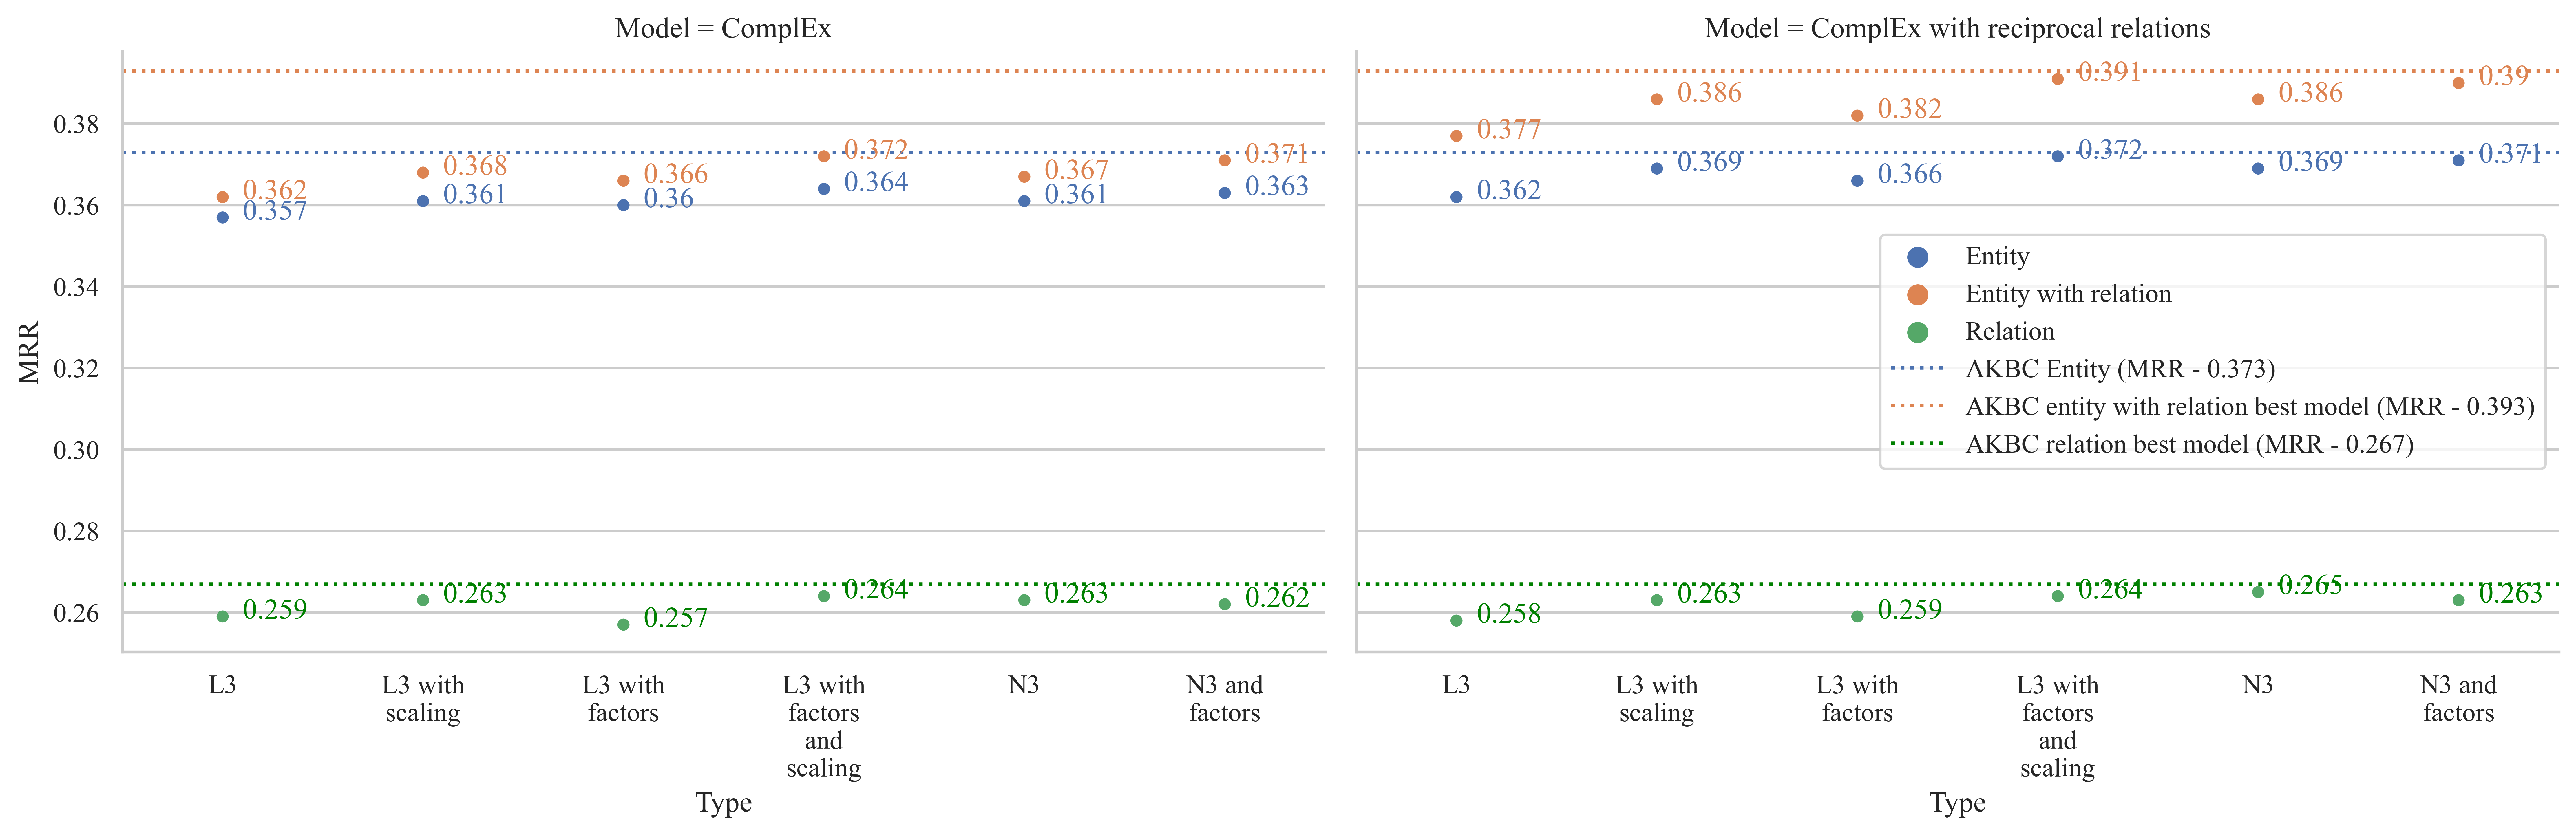
\includegraphics[width=\linewidth]{Images/Ablation_FB237.png}
	\caption[Performance of model when applying changes on FB15K-237]{Performance of model when applying changes on FB15K-237. \textit{Type:} indicates the changes has been applied}
	\label{fig:Ablation FB237}
	\end{center}
\end{figure}


The results for ablation study are shown in Figures \ref{fig:Ablation FB237} and \ref{fig:Ablation WNRR} respectively. The orange represents the performance of models trained on hybrid training objective, while the blue represent for models trained on standard training objective. The green is for models trained on relation training objective. The lines illustrate the performance from \citet{chen2021relation}'s models. The "type"-axis represents the changes that were applied to the models. "Normal weight" means that models were trained with the same-value weights as reported in the papers. "Scaled weight" means the regularization weights were scaled based on the difference in the implementation between two codebases. "Complex emb. vector" means that embedding vectors were considered as complex vector when performing penalty calculation.


On FB15K-237, the Figure \ref{fig:Ablation FB237} demonstrates, by using reciprocal relation technique, the performance of model on entity prediction (entity MRR) was boosted, i.e., MRR increases 1\% or 2\% (from 36.2\% to 37.7\%). Furthermore, with unexplored regularization weights, the models could achieve must more better results (37.7\% to 38.6\% MRR). 

However, the main difference between LibKGE and \citet{chen2021relation}'s codebase, i.e., considering embedding vector as complex vectors could slightly improve MRR by around 0.5\%. Clearly seen that, the main improvement comes from unexplored regularization weights and it does not matter how we treat the embedding vector as complex vector or not. 

\begin{figure}[!htbp]
	\begin{center}
	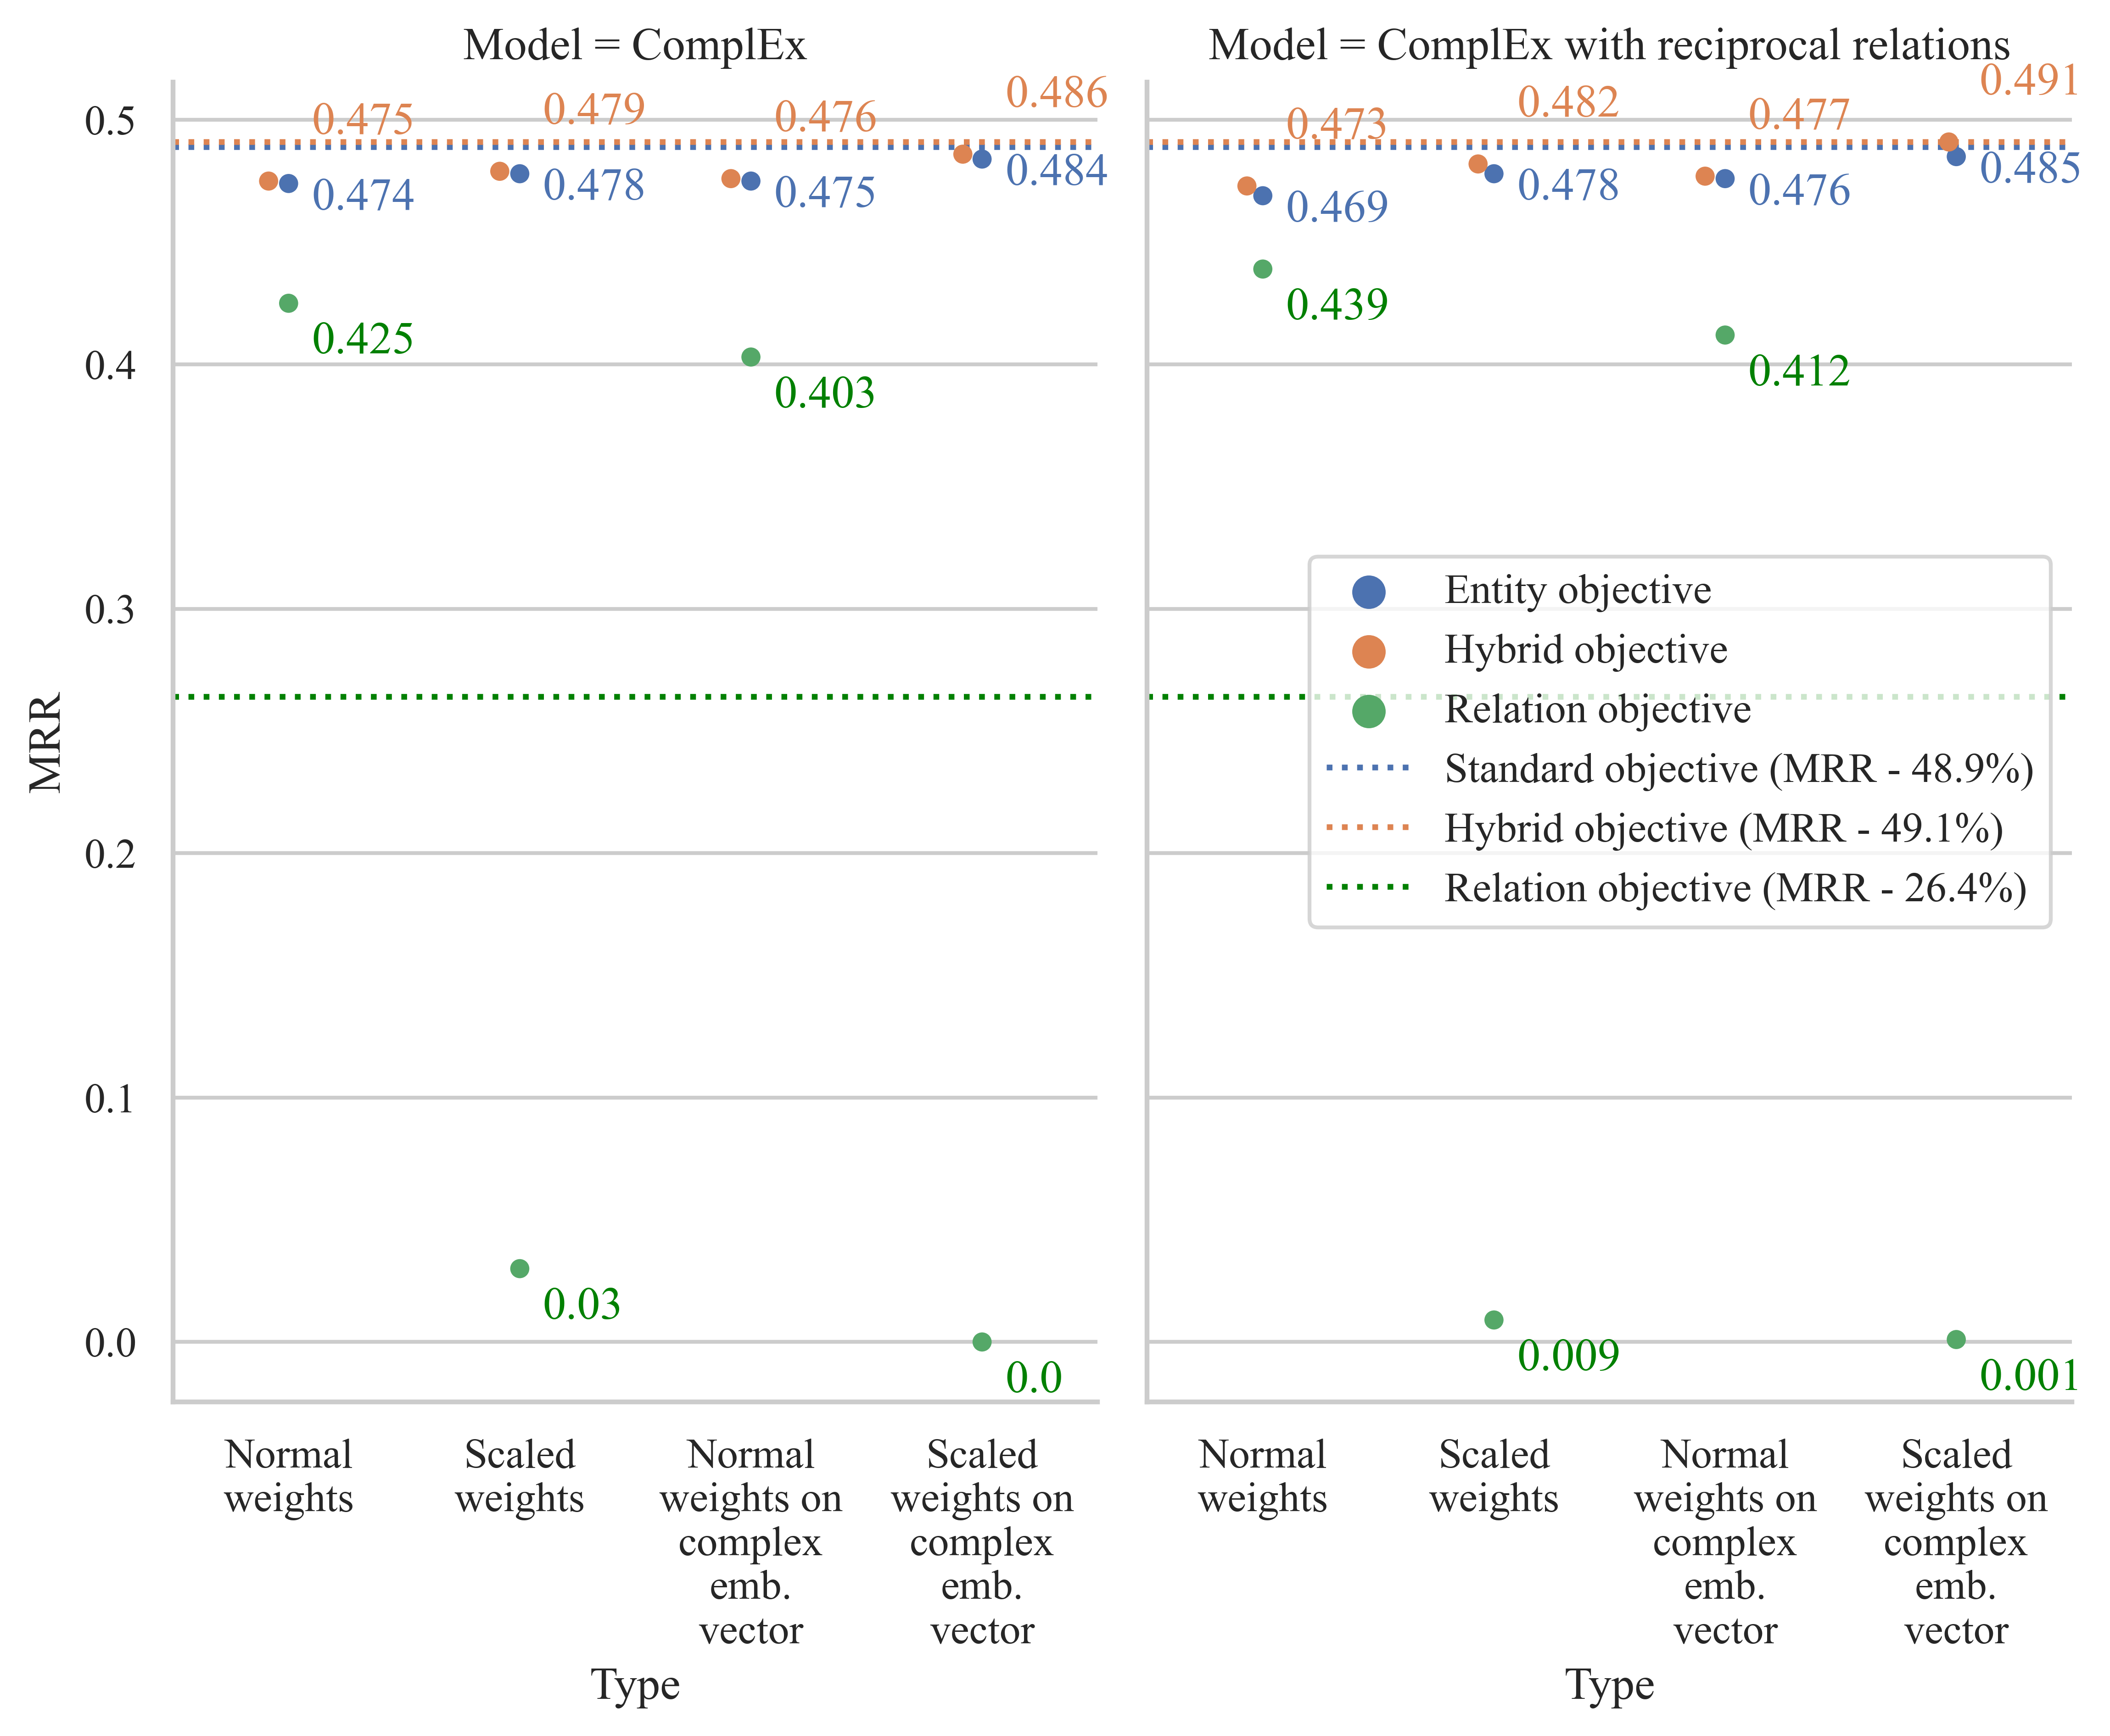
\includegraphics[width=\linewidth]{Images/Ablation_WNRR.png}
	\caption[Performance of model when applying changes on WN18RR]{Performance of model when applying changes on WN18RR. \textit{Type:} indicates the changes has been applied}
	\label{fig:Ablation WNRR}
	\end{center}
\end{figure}

On WN18RR, Figures \ref{fig:Ablation WNRR} states that the improvement is not really clear. However, we can see the same pattern as we observed on FB15K-237, with the unexplored regularization weights, the model trained on standard and hybrid objectives could achieve much more better results in entity MRR, that is 48.6\% and 48.4\% vs 47.6\% and 47.5\% without reciprocal technique and 49.1\% and 48.5\% vs 47.7\% and 47.6\% with reciprocal relations.
\newline

\noindent\textbf{Complex embedding vector in unrestricted HPC space.} The HPC space from \citet{chen2021relation} is a restricted space with numerous predefined hyperparameters such as regularizer, embedding initialization method or training optimizer. Therefore, we conducted an experiment on an unrestricted HPC space to observe the effect of considering embedding vectors as complex vectors in penalty calculation. The unrestricted HPC space we chose is from \citet{Ruffinelli2020You}. 

\begin{table}[!htbp]
\centering
\resizebox{\textwidth}{!}{%
\begin{tabular}{@{}lcccllll@{}}
\toprule
\textbf{Dataset} & \multicolumn{1}{l}{\textbf{Relation}} & \multicolumn{1}{l}{\textbf{Entity}} & \textbf{Complex vector} & \textbf{MRR} & \textbf{Hits@1} & \textbf{Hits@3} & \textbf{Hits@10} \\ \midrule
FB15K-237 & No & Yes & Yes & 34.9 & 26.2 & 38.0 & 52.3 \\
 & No & Yes & No & 35.0 & 26.1 & 38.3 & 52.8 \\ \cmidrule(l){2-8} 
 & Yes & Yes & Yes & 35.0 & 26.6 & 38.0 & 51.5 \\
 & Yes & Yes & No & 35.1 & 26.4 & 38.2 & 52.9 \\ \midrule
WN18RR & No & Yes & Yes & 47.6 & 44.5 & 48.6 & 54.0 \\
 & No & Yes & No & 47.6 & 44.4 & 48.9 & 53.8 \\ \cmidrule(l){2-8} 
 & Yes & Yes & Yes & 46.2 & 43.5 & 47.3 & 51.2 \\
 & Yes & Yes & No & 46.5 & 43.9 & 47.5 & 51.5 \\ \bottomrule
\end{tabular}%
}
\caption[Effect of considering embedding vectors as complex vectors]{The performance of models in FB15K-237 and WN18RR with and without considering embedding vectors as complex vectors. The \textit{Complex vector} indicates that considering the embedding vector as complex vector in penalty calculation. \textit{Yes} value means model considered embedding vectors as complex vectors while \textit{No} value means model does not consider embedding vectors as complex vectors. }
\label{tab:ICLR factor matter}
\end{table}

Table \ref{tab:ICLR factor matter} reports the models' performance with and without considering embedding vectors as complex vectors on unrestricted HPC space. From the table we can note that there is no difference between with or without the consideration. Therefore the main improvement come from unexplored values in the HPC space. 

\section[Finding ability of LibKGE]{Ability of finding \cite{chen2021relation}'s best models}

In this chapter, we reported the differences between two codebase and we have found exactly the configuration to reproduce the best models from \cite{chen2021relation} using LibKGE. However, the main question now is that we can find those models using Random Search approach in LibKGE or those models that are too good to be found. 

\begin{table}[!htbp]
\centering
\resizebox{0.9\textwidth}{!}{%
\begin{tabular}{@{}llll@{}}
\toprule
Trial & Hyperparameter & Values & entity MRR \\ \midrule
1 & Embedding initialization & Normal & 39.1 \\
 & Std. deviation (Normal) & 0.001 &  \\
 & Lp regularization & L3 &  \\
 & Entity emb. weight & {[}0.0005, 1.0{]}, log scale &  \\
 & Relation emb. weight & {[}0.0005, 1.0{]}, log scale &  \\ \midrule
2 & Embedding initialization & Normal & 39.0 \\
 & Std. deviation (Normal) & 0.001 &  \\
 & Lp regularization & \{L1, L2, L3, None\} &  \\
 & Entity emb. weight & {[}0.0005, 1.0{]}, log scale &  \\
 & Relation emb. weight & {[}0.0005, 1.0{]}, log scale &  \\ \midrule
2 & Embedding initialization & Normal & 38.9 \\
 & Std. deviation (Normal) & 0.001 &  \\
 & Lp regularization & \{L1, L2, L3, None\} &  \\
 & Entity emb. weight & {[}0.0005, 1.0{]}, log scale &  \\
 & Relation emb. weight & {[}0.0005, 1.0{]}, log scale &  \\ \bottomrule
\end{tabular}%
}
\caption[Model performance when relaxing the restricted HPC space]{Model performance when relaxing the restricted HPC space. \textit{Trial} indicates the id of trial, \textit{Hyperparameters} are the hyperparameters we attempted to relax with their correspoding values in \textit{Value} column. Entity MRR indicates the MRR that best model can achieved.}
\label{tab:finding ability}
\end{table}

Due to the huge difference between restricted HPC space from \cite{chen2021relation} and unrestricted HPC space from \cite{Ruffinelli2020You}, we relaxed the hyperparameter bit by bit. Within this scope of study, we only focus on reproducing the model trained on hybrid training objective, the best-performance model was selected on entity MRR. The model was trained on FB15K-237. The table \ref{tab:finding ability} shows the performance of the best models we found after 3 times relaxing the restricted HPC space (on entity MRR). 

As illustrated in the table, so far we still can find the best model from \cite{chen2021relation}. However, the range for regularization weight is still small $[0.0005, 1.0]$ compared to unrestricted HPC space i.e., close interval $[1.0^{-20}, 1.0^{-01}]$. Therefore, the future study should enlarge the close interval for regularization weight to test the finding ability of LibKGE.
